\section{Programmierung}

\begin{tabularx}{\columnwidth}{|p{4cm}|X|}
	\hline
	\textbf{Abschnitt} & \textbf{Inhalt}\\
	\hline
	\textbf{Name} & \\
	\hline
	\textbf{Autor(en)} & \\
	\hline
	\textbf{Priorität} & \\	
	\hline	
	\textbf{Kritikalität} &\\
	\hline
	\textbf{Quelle} & \\
	\hline
	\textbf{Verantwortlicher} & \\
	\hline
	\textbf{Kurzbeschreibung} & \\
	\hline
	\textbf{Auslösendes Ereignis} & \\
	\hline
	\textbf{Akteure} & \\
	\hline
	\textbf{Vorbedingung} & \\
	\hline
	\textbf{Nachbedingung} & \\
	\hline
	\textbf{Ergebnis} & \\
	\hline
	\textbf{Hauptszenario} &\\
	\hline
	\textbf{Alternativszenario} & \\
	\hline
	\textbf{Ausnahmeszenario} & \\
	\hline
	\textbf{Qualitäten} & \\
	\hline
\end{tabularx}
\captionof{table}{}
\label{tab:}

\newpage
%%[width=\textwidth]
%\begin{figure}[h]
%	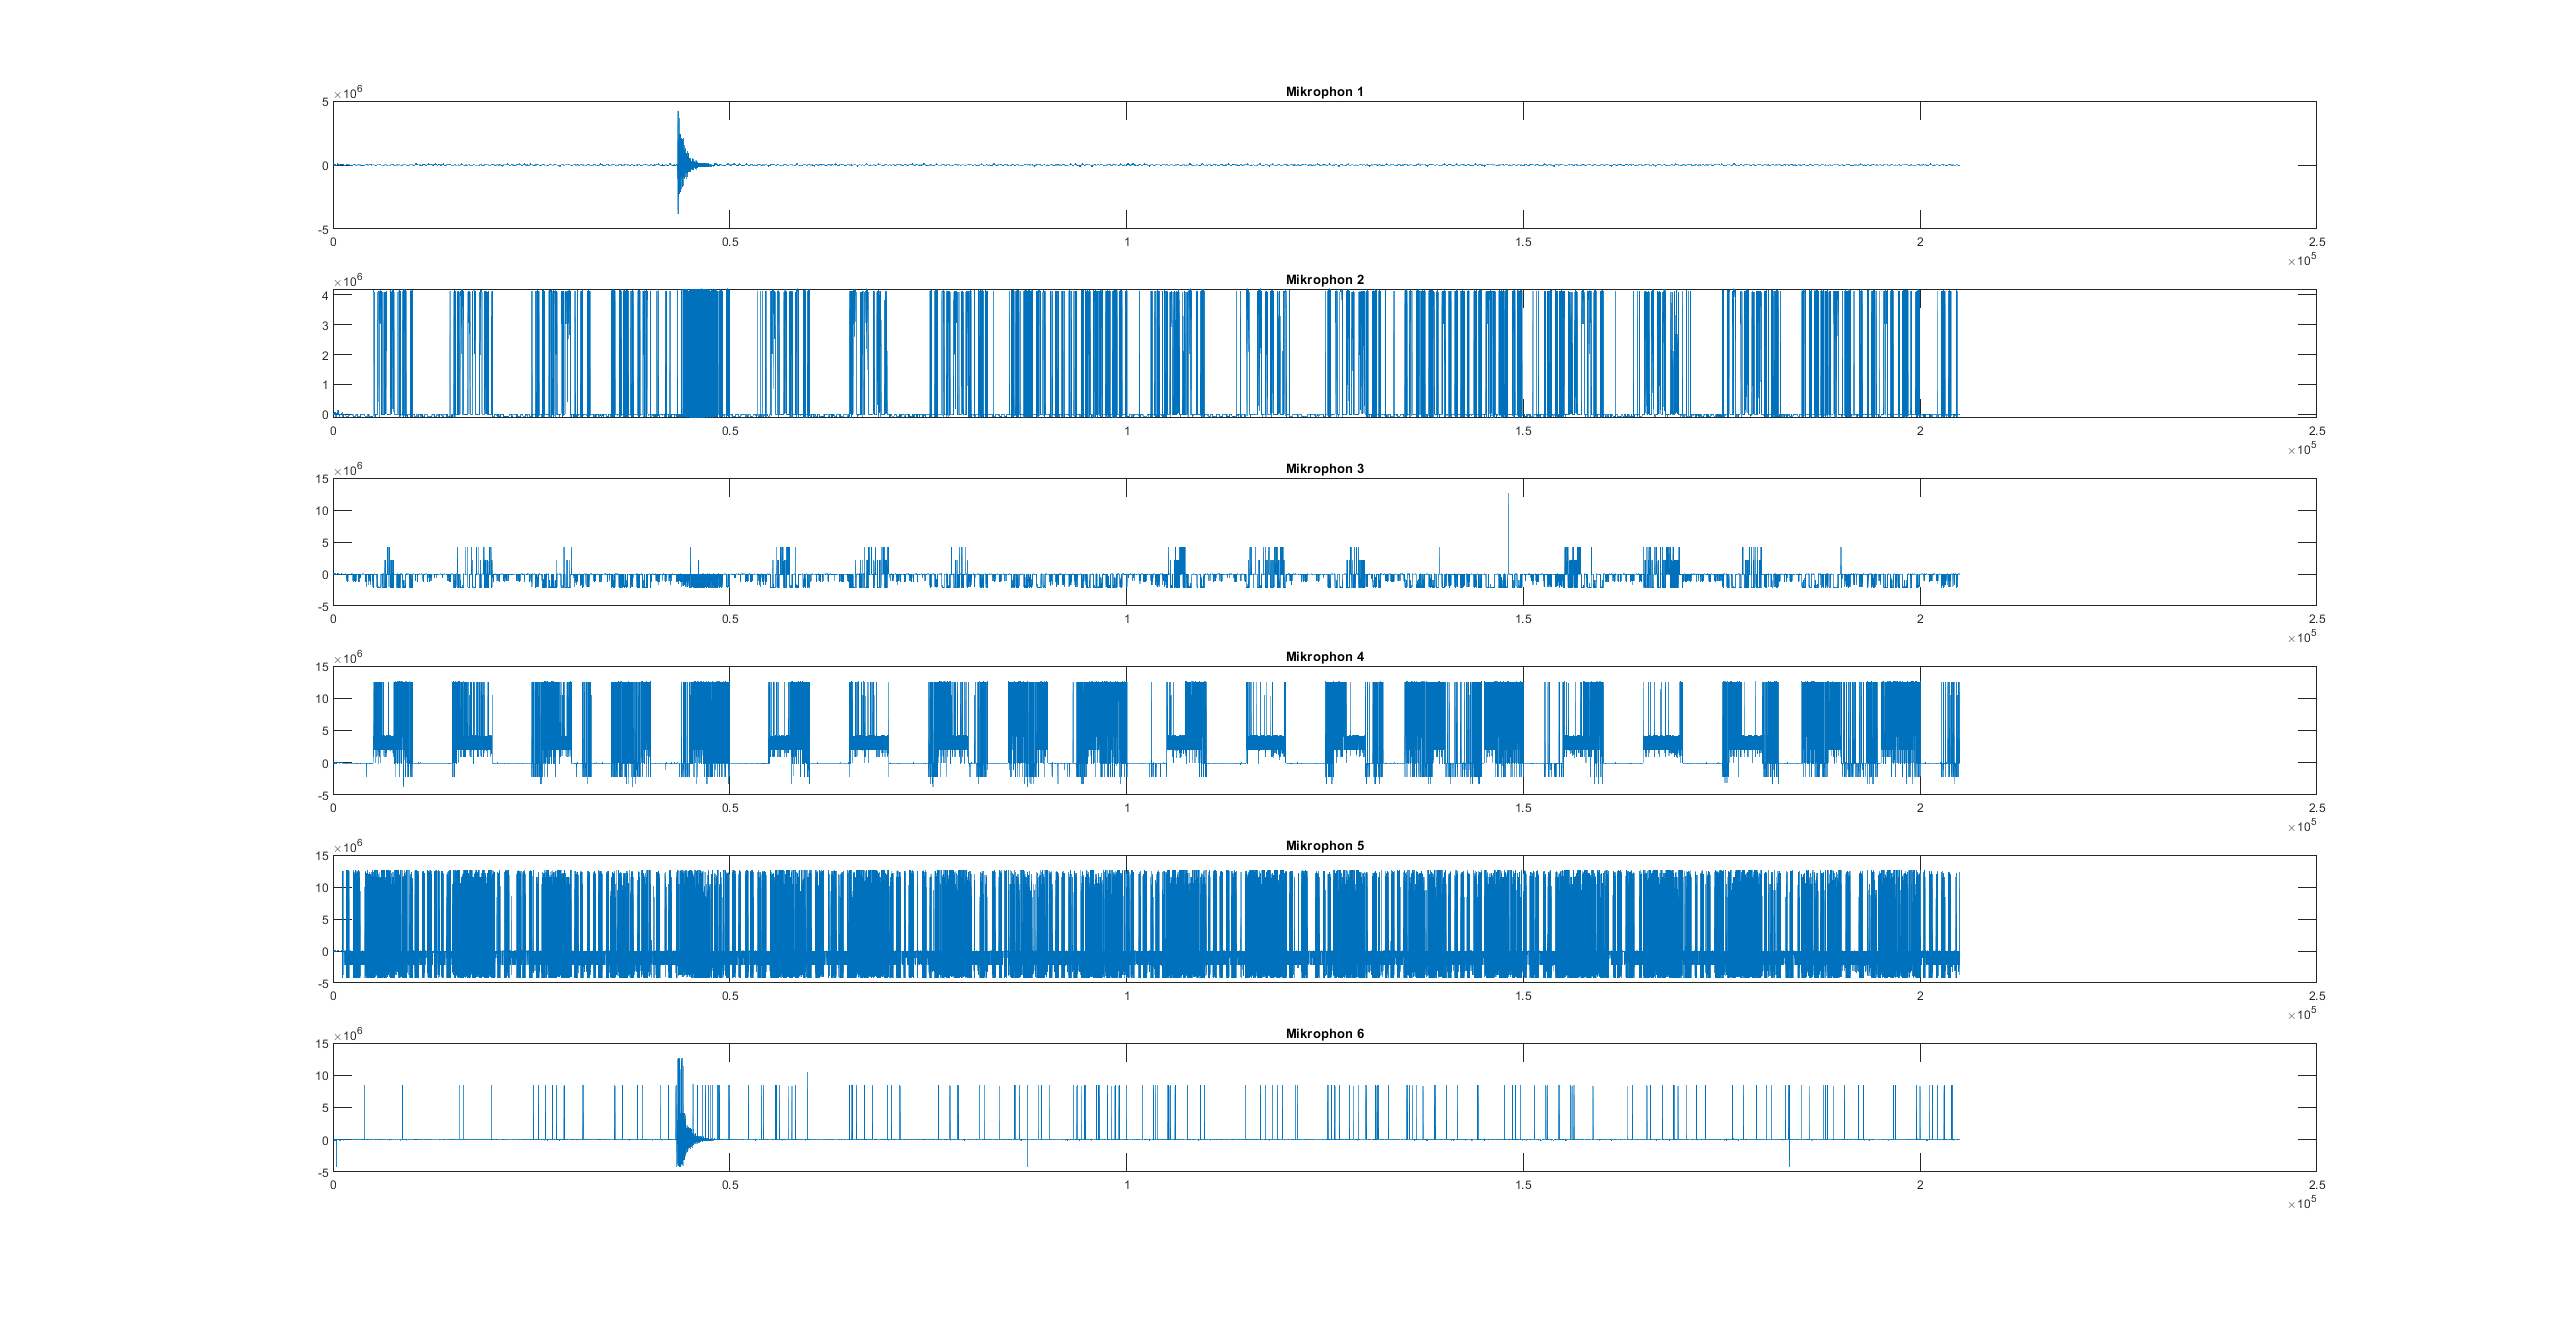
\includegraphics[scale=0.1]{Sections/Programmierung/Test_1}
%	\caption{Test 1}
%	\label{fig:Test_1}
%\end{figure}
%
%\begin{figure}[t]
%	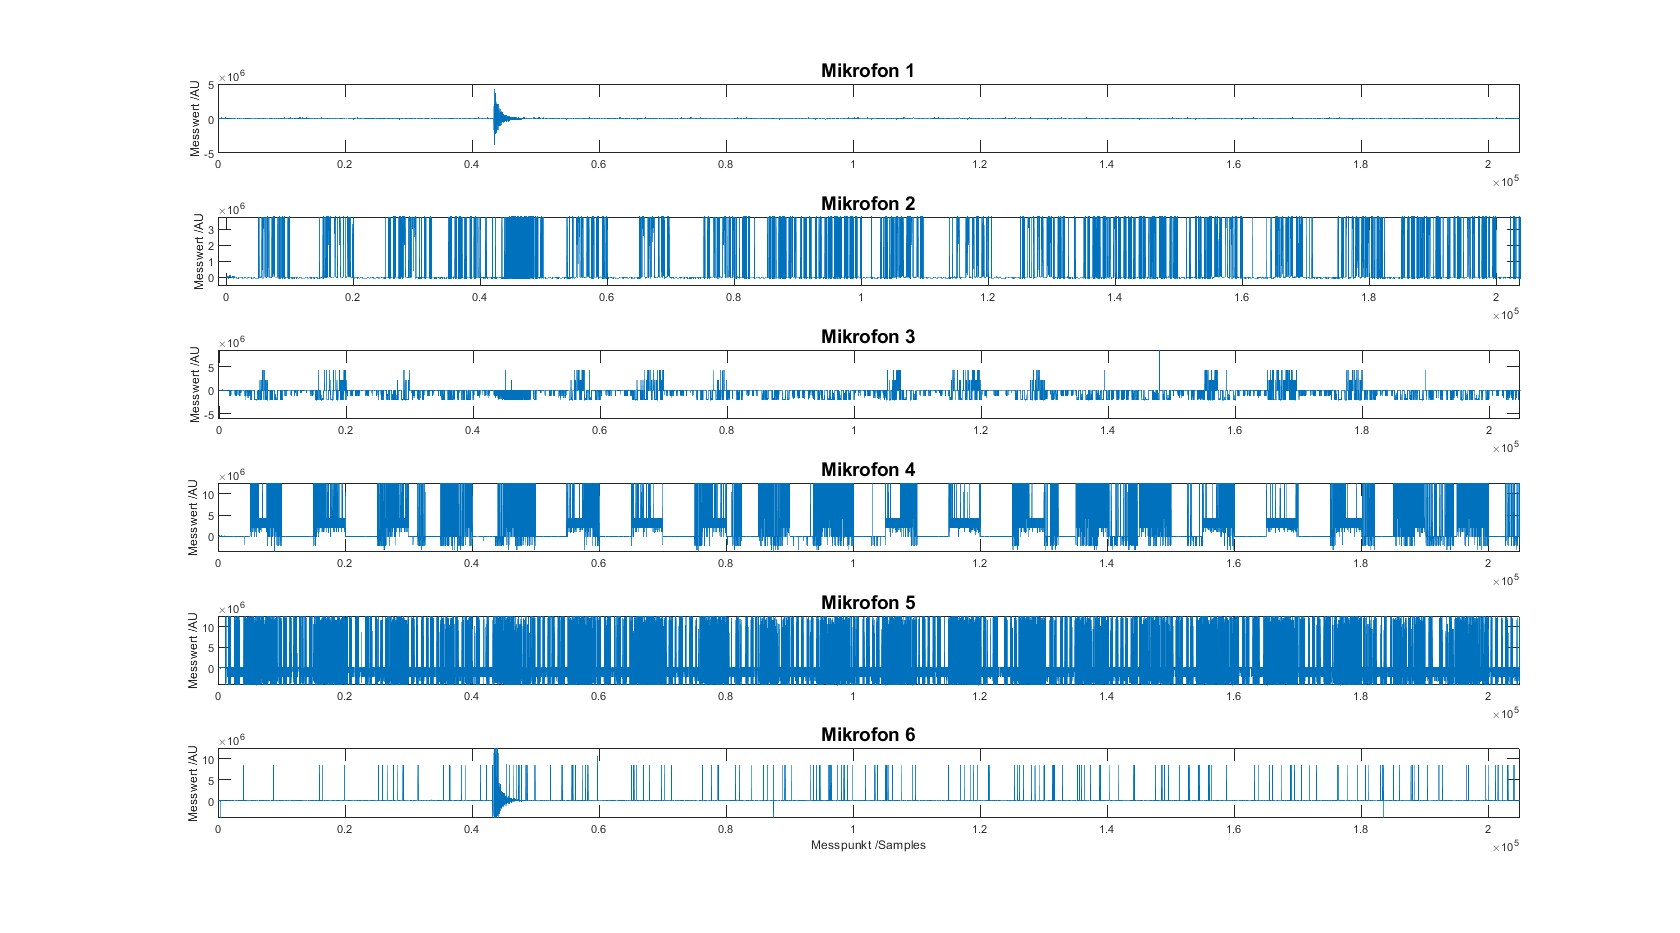
\includegraphics[scale=0.1]{Sections/Programmierung/Test_1_b}
%	\caption{Test 1 b}
%	\label{fig:Test_1_b}
%\end{figure}

\begin{figure}[h]
	\begin{center}
		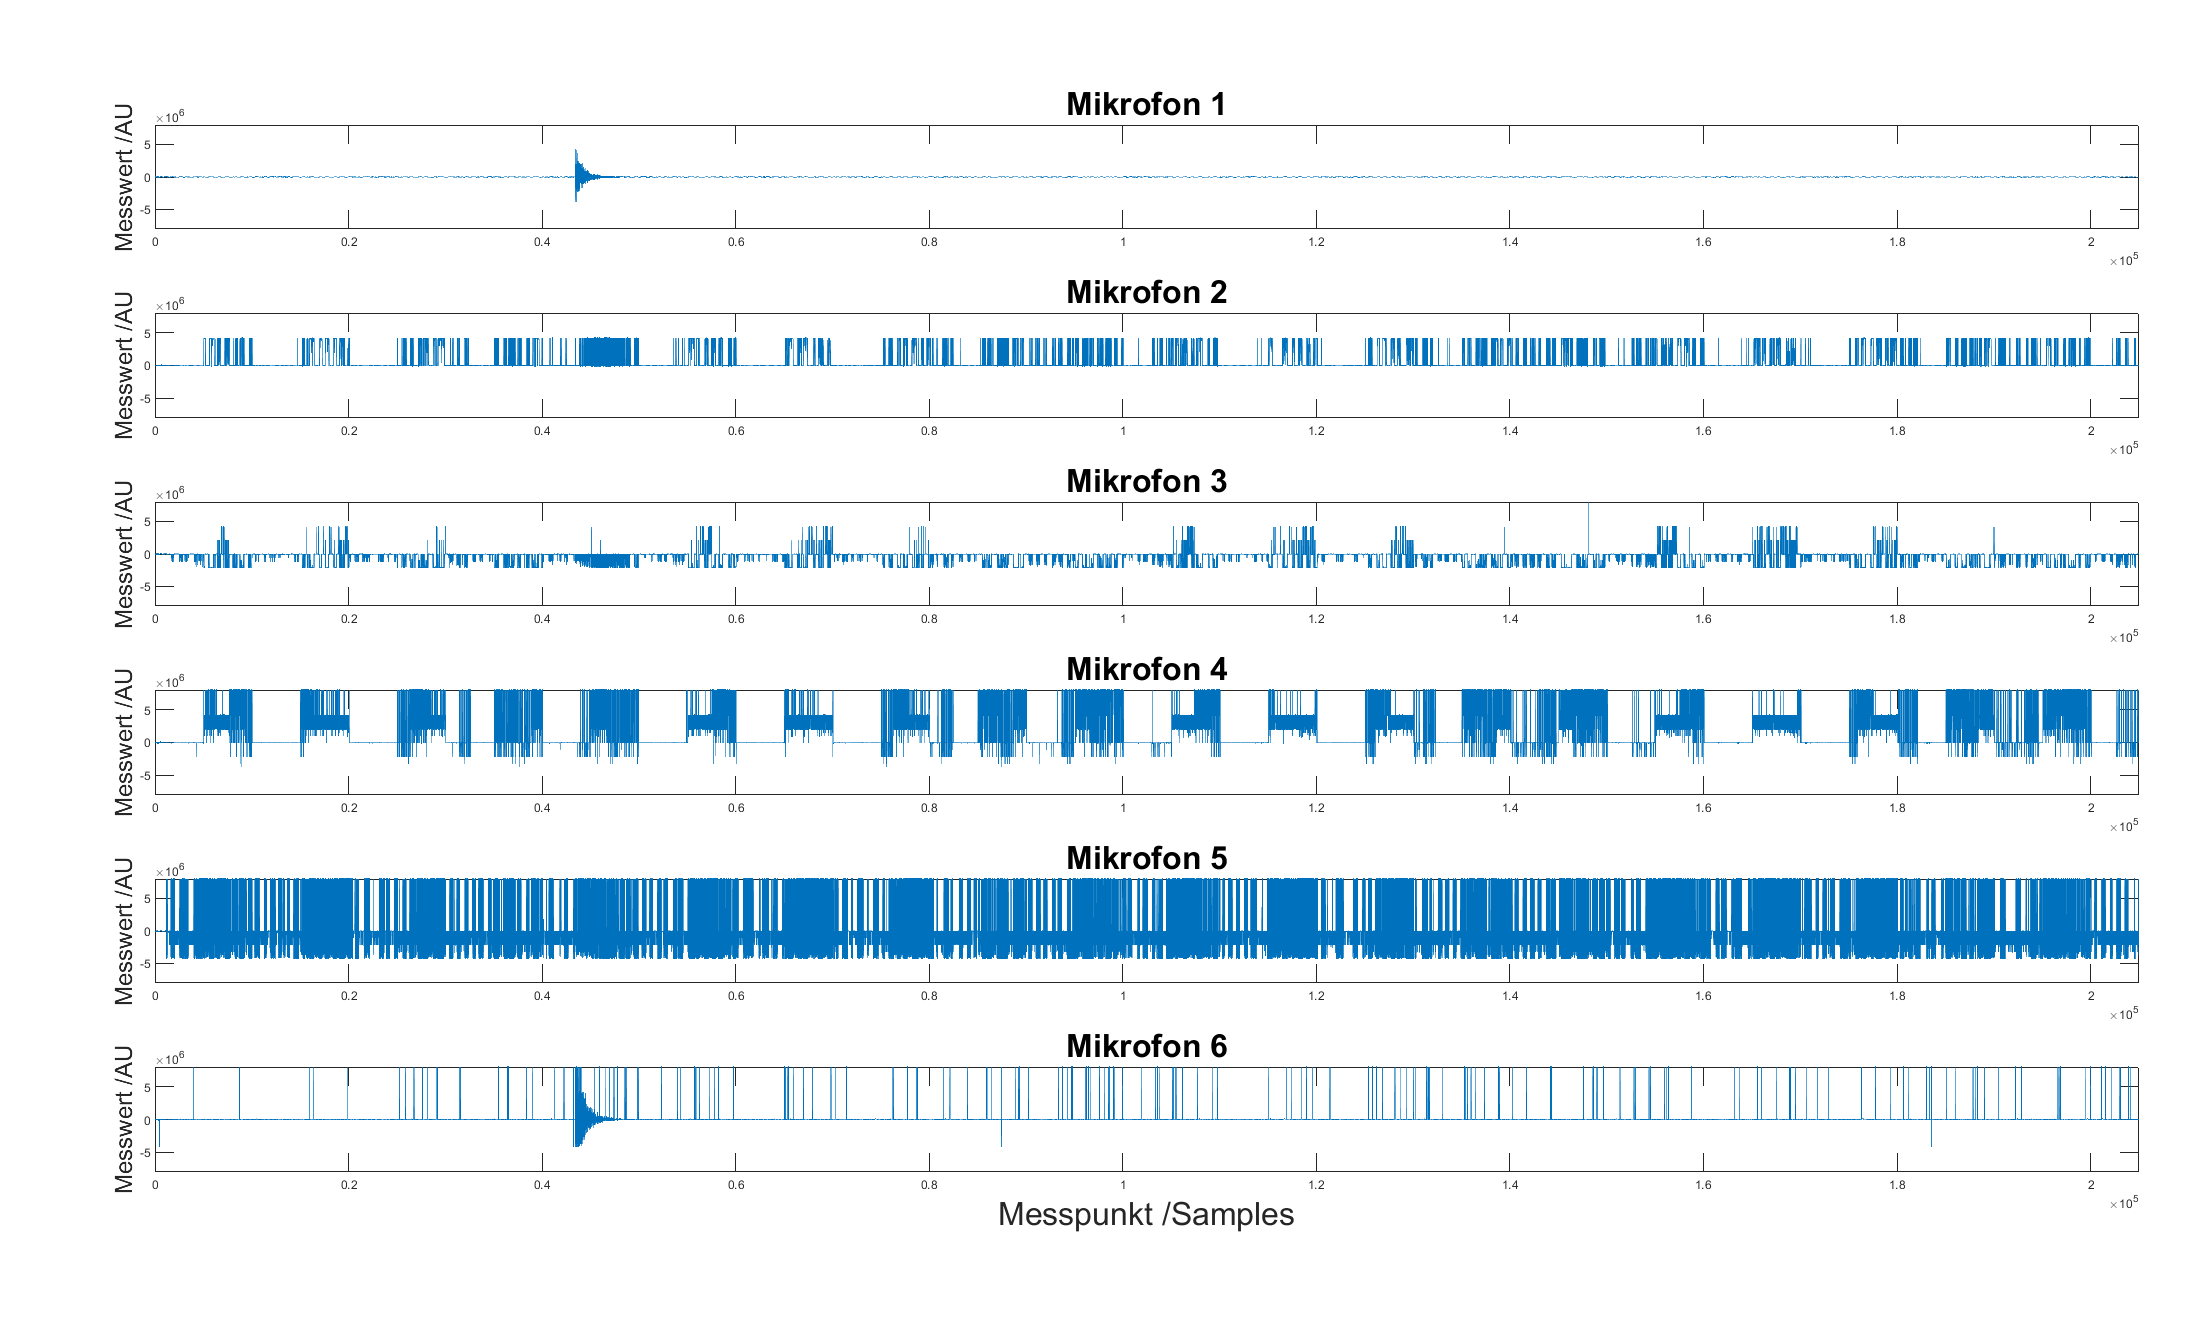
\includegraphics[width=\textwidth]{Sections/Programmierung/Test_1_d}
	\end{center}
	\caption{Test 1 b}
	\label{fig:Test_1_b}
\end{figure}

\begin{figure}[h]
	\begin{center}
		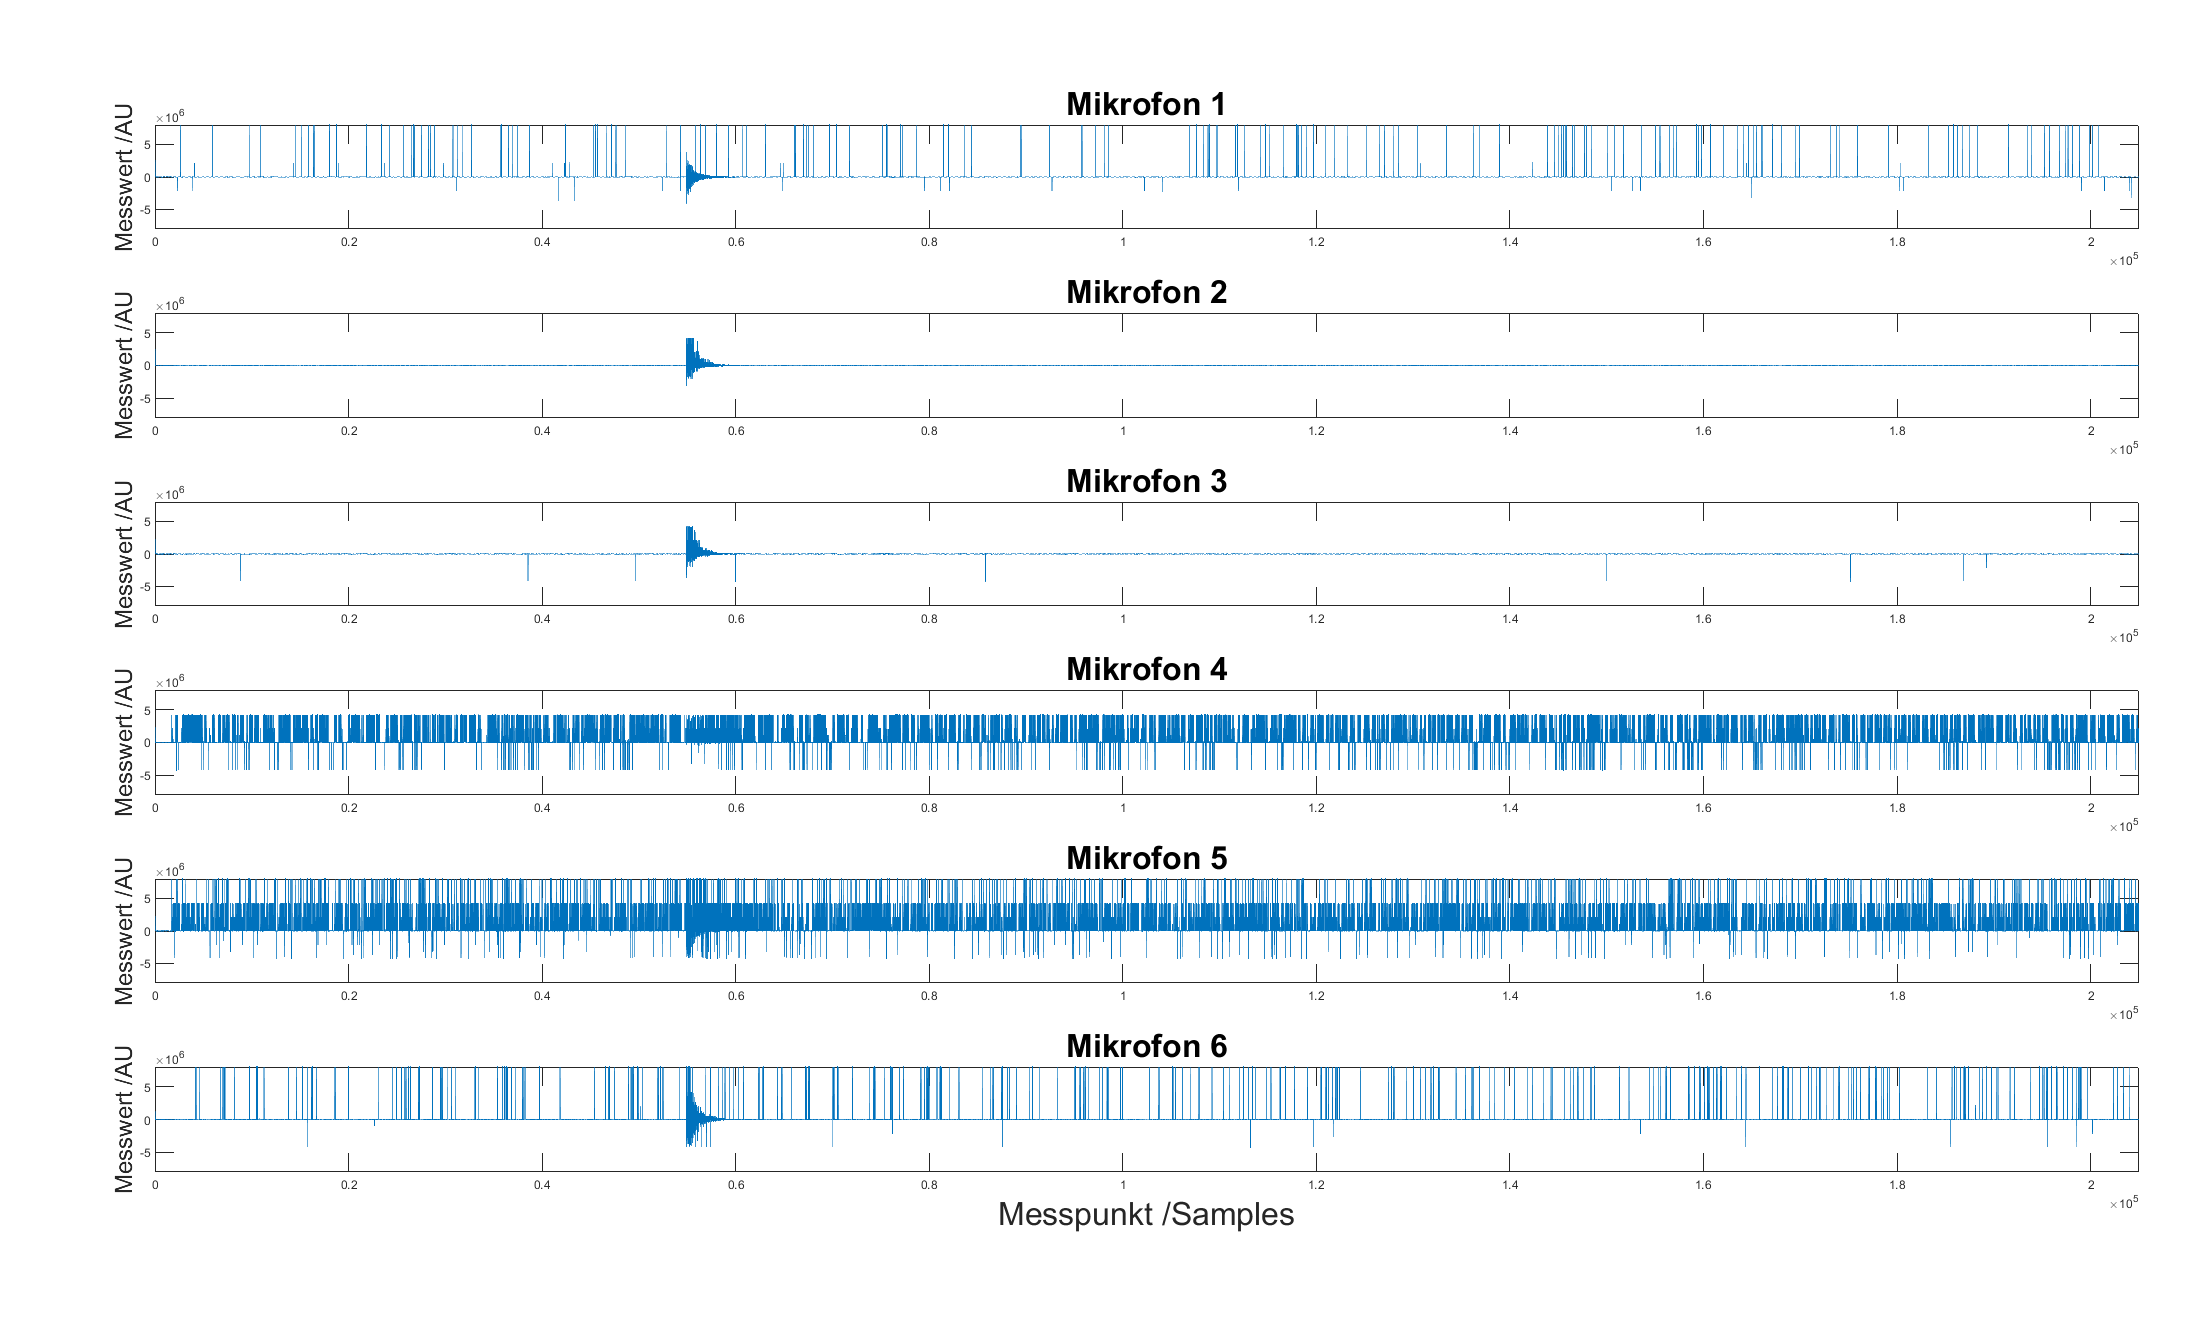
\includegraphics[width=\textwidth]{Sections/Programmierung/Test_2_d}
	\end{center}
	\caption{Test 2 d}
	\label{fig:Test_2_d}
\end{figure}

\begin{figure}[h]
	\begin{center}
		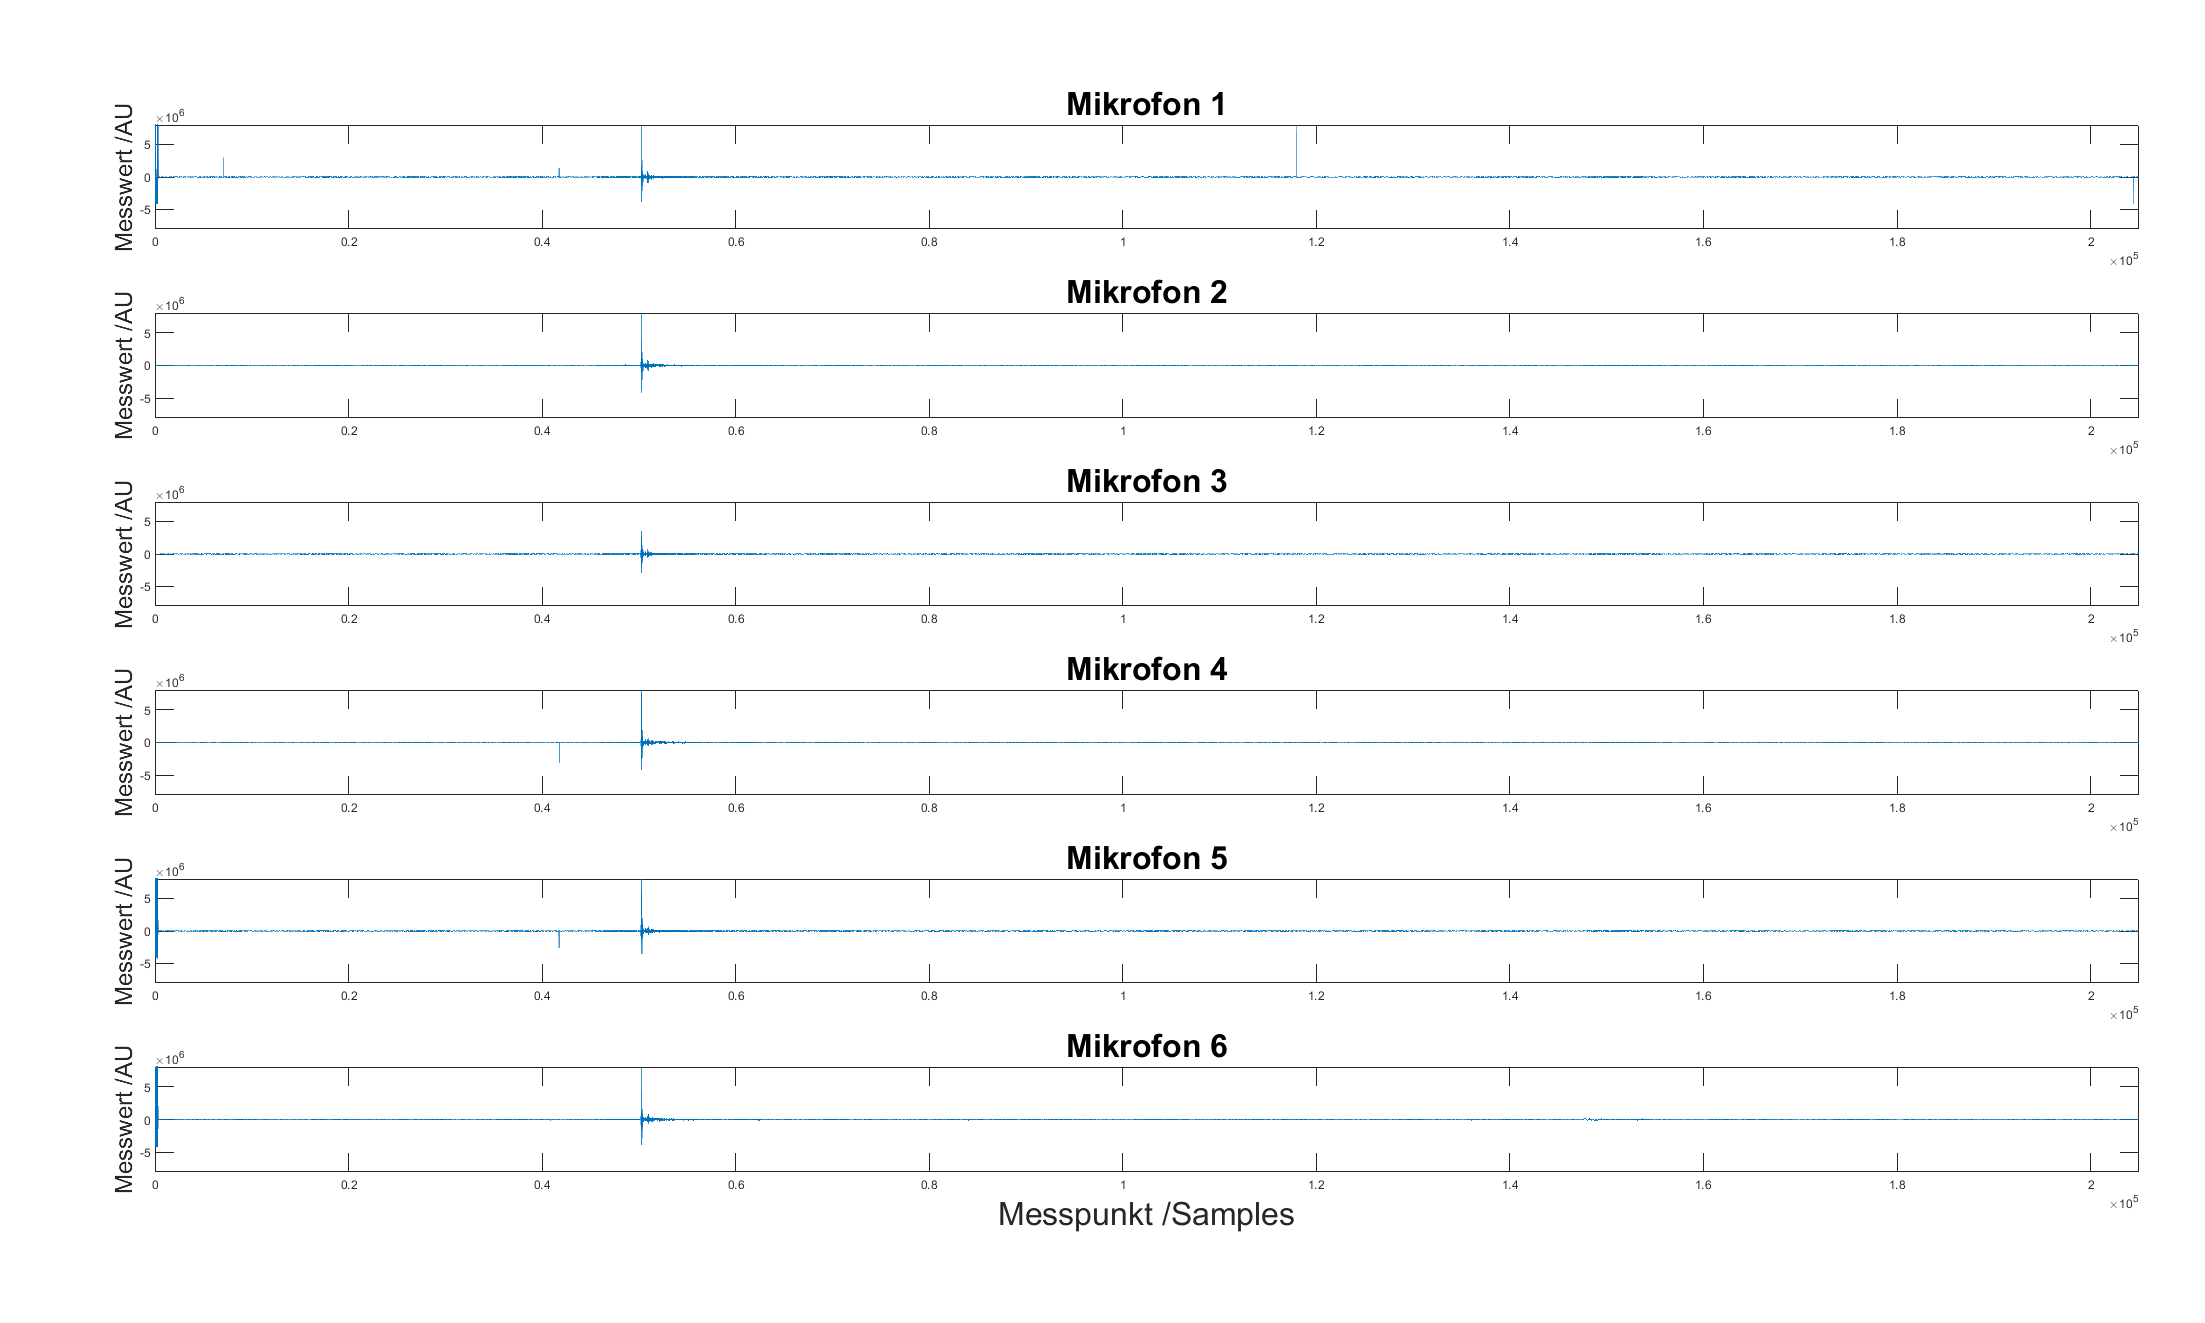
\includegraphics[width=\textwidth]{Sections/Programmierung/Test_3_d}
	\end{center}
	\caption{Test 3 d}
	\label{fig:Test_3_d}
\end{figure}

\newpage